\defcitealias{ali_et_al2015}{A15}

\chapter{PAPER-64}
\label{c.PSA64}


\section{Overview}
\label{sec:PSA64overview}

In the previous chapter we have discussed three overarching 21\,cm power spectrum themes --- signal loss, error estimation, 
and bias. Understanding the subtleties and trade-offs involved in each is necessary for an accurate and robust understanding of 
a power spectrum result. 

We now apply these lessons to data from the PAPER experiment in order to illustrate our revised analysis pipeline. We begin with a brief overview of PAPER's data processing steps prior to power spectrum estimation before delving into each theme in detail.

\subsection{Observations}

As described in Chapter \ref{sec:PAPER_intro}, PAPER is a dedicated 21\,cm experiment located in the Karoo Desert in South Africa. The PAPER-64 configuration consists of 64 dual-polarization drift-scan elements that are arranged in a grid layout (Figure \ref{fig:ant_layout}). While every unique baseline is used for calibration, only a subset of the baselines are used for the power spectrum analysis in \citetalias{ali_et_al2015} (the three baselines used are the $30$\,m East/West baselines and their off-diagonal companions where two antennas are in adjacent columns and neighboring rows) and only one baseline-type is used for the demonstrations in this chapter (only the $30$\,m East/West baselines).

PAPER-64 conducted nighttime observations from November 2012 to March 2013. Over the course of the season, LST-coverage varied slightly, with power spectrum analyses focusing on the ``cold patch" range from $\sim0$-$8$\,hours when the Galaxy is below the horizon. The PAPER correlator processes a 100-200\,MHz bandwidth that consists of 1024 channels, each of width 97.6\,kHz. Visibilities are integrated for 10.7\,s before being written to disk. 

PAPER's raw data is compressed by a factor of $\sim70$ through the use of RFI, delay, and delay-rate filters. More specifically, radio frequency interference is flagged at the $6\sigma$ level. Next, a low-pass delay filter is applied to all the data in order to filter out delays greater than the maximum delay allowed by the longest baseline in the array. Similarly, a low-pass fringe-rate, or delay-rate filter is applied to limit fringe-rates to allowable scales set by the array. Finally, the data is decimated to critical Nyquist sampling rates of 493\,kHz and 42.9\,s. For more details about PAPER's data acquisition and compression pipelines, we refer the reader to \citet{parsons_et_al2010} and \citetalias{ali_et_al2015}.

\begin{figure}
    \centering
    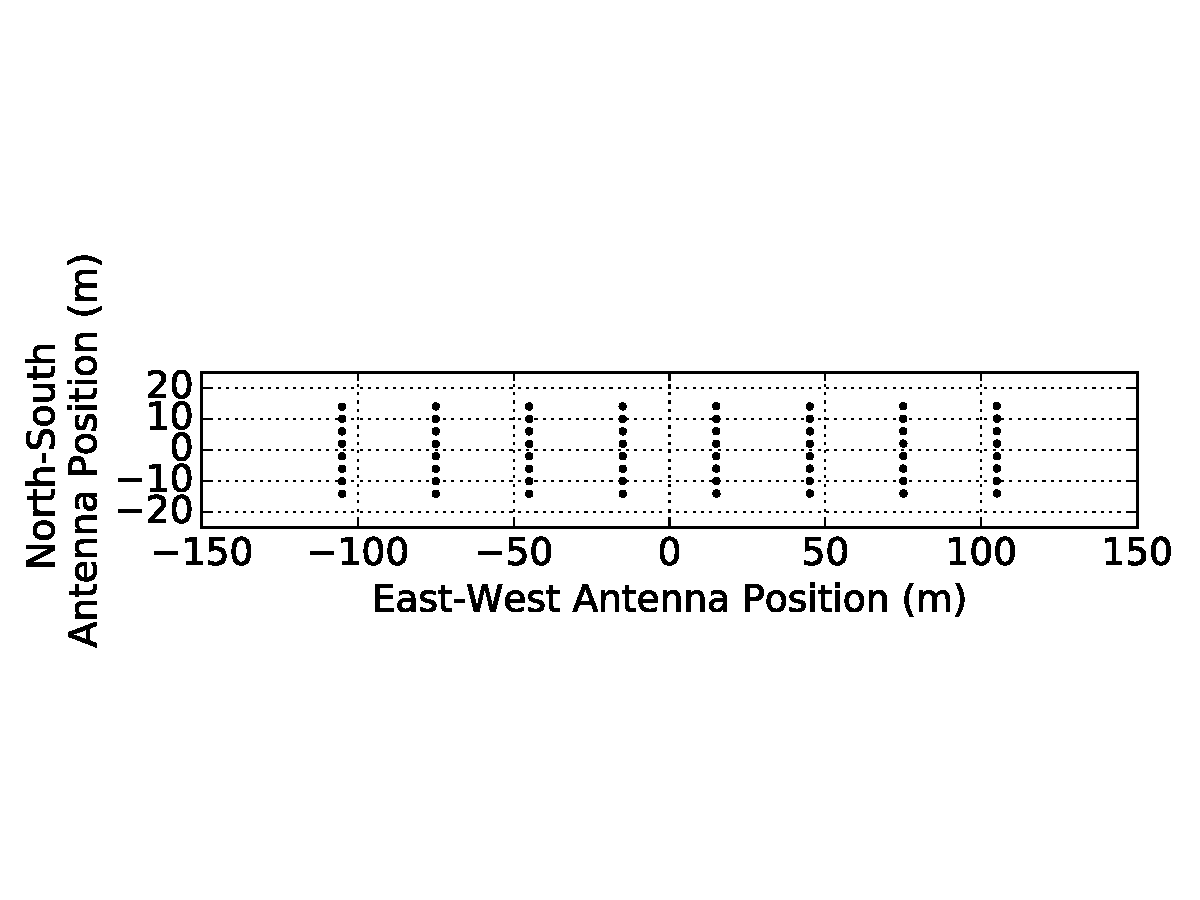
\includegraphics[trim={0cm 4.5cm 0cm 4.5cm},width=\columnwidth]{plots/ant_layout_aspect.pdf}
    \caption{The PAPER-64 antenna layout. We use only $10$ of the $30$ m East/West baselines for the analysis in this 
paper (i.e., a subset of the shortest horizontal spacings).}
    \label{fig:ant_layout}
\end{figure}

\subsection{Data Processing}
\label{sec:PSA64_processing}

As described in Chapters \ref{sec:calibration_intro}, \ref{sec:fg_intro}, \ref{sec:frf_intro}, the primary post-processing steps of PAPER's compressed data is calibration, foreground-filtering, and fringe-rate filtering. We now give a brief overview of each, as applied to PAPER data.

We employ the package {\sc Omnical} for redundant calibration (\citealt{zheng_et_al2014}), which comprises of three steps. The first is {\tt FirstCal}, which uses all baseline redundancies to generate a static gain solution for each antenna that will unwrap any phase wrapping between two identical baselines. We perform {\tt FirstCal} because the next stage of {\sc Omnical} cannot tell the difference between a phase of $0$ and $2\pi$, for example. The second step is {\tt LogCal}, which takes the log of all the visibility equations (Equation \eqref{eq:gains}) and separates the real and imaginary components into two matrices. Coarse solutions are determined for both the antenna gains and ``model" visibilities (one for each baseline type) simultaneously. The final step of {\sc Omnical} is {\tt LinCal}, which applies small perturbations to the {\tt LogCal} solutions in an iterative fashion, honing in on the optimal solutions.
 
It is important to note that while {\sc Omnical} is powerful for ensuring array redundancy, it is not able to solve for $4$ calibration parameters - namely, the overall gain, phase, and tip/tilt of the array. For absolute calibration, we turn to a standard self-calibration routine which includes imaging Pictor A, Fornax A, and the Crab Nebula in order to fit for the overall phase solutions and the flux scale.

After calibration, we combine the XX and YY linear polarization data to form pseudo-Stokes I as defined as:

\begin{equation}
V_{I} = \frac{1}{2}(V_{XX}+V_{YY})
\end{equation}
(\citealt{moore_et_al2013}).

Next, a delay-filter is used to filter out foregrounds contained inside the maximum delay set by each baseline. This is accomplished by de-convolving out our sampling function (which contains flags due to RFI) from our delay-domain visibilities using a CLEAN-like algorithm that restricts our clean components to inside the horizon limit, plus a 15\,ns buffer. The Fourier-transformed clean components are then subtracted from our visibilities. This filtering process is performed on a per-baseline, per-integration basis, and we achieve a brightness suppression of $\sim4$ orders of magnitude in our visibilities.

After delay-filtering, we perform a final round of RFI-removal by flagging visibilities that lie more than $3\sigma$ above the mean on a time, frequency, and baseline basis. Finally, we stack our data in LST into two datasets, alternating between even and odd Julian Dates to create an ``even" and ``odd" LST-binned dataset. A total of 124 days of data are included in the LST-binned dataset.

The final step before power spectrum estimation is fringe-rate filtering. The chosen filter (which is described in the next section) is applied on a per-baseline basis and weights the fringe-rate bins on the sky by the RMS of the primary beam at that same location. A smooth filter is constructed by fitting a Gaussian to the filter shape in the fringe-rate domain. Additionally, fringe-rates below 0.2\,mHz are zeroed out, effectively removing slowly-varying signals such as crosstalk. We then convolve our time-domain visibilities by the Fourier-transform of the fringe-rate filter to yield time-averaged visibilities that have gained another order of magnitude in sensitivity.

\subsection{Case Study Data}

For the case study presented in the rest of this chapter, we 
focus on a subset of the PAPER-64 data used in \citetalias{ali_et_al2015}, namely, on LST-binned, Stokes I estimated data \citep{moore_et_al2013} from PAPER's $30$ m East/West baselines (Figure 
\ref{fig:ant_layout}). Hence, all data processing steps are identical to those in \citetalias{ali_et_al2015} until after the LST-binning step in Figure 3 of \citetalias{ali_et_al2015}.

The previously best published 21\,cm upper limit result from \citetalias{ali_et_al2015} placed a $2\sigma$ upper limit 
on $\Delta^{2}(k)$, defined as

\begin{equation}
\Delta^{\textbf{2}}(k) = \frac{k^{3}}{2\pi^{2}}\,\hat{P}(k),
\end{equation}

\noindent of $(22.4$ mK$)^{2}$ in the range $0.15 < k < 0.5$\,$h$ Mpc$^{-1}$ at $z = 8.4$. The need to revise this limit stems mostly from previously under-estimated signal loss and under-estimated error bars, both of which we 
address in the following sections. 

For the analysis in this paper, we use $8.1$ hours of LST, namely an RA range of $0.5$-$8.6$ hours (\citetalias{ali_et_al2015} uses a slightly longer RA 
range of $0$-$8.6$ hours; we found that some early LSTs were more severely foreground contaminated). We also use only $10$ baselines, a subset of the $51$ total East/West baselines used in \citetalias{ali_et_al2015}, in order to illustrate our revised methods. All power spectrum results are produced for a center frequency of 151\,MHz using a width of 10\,MHz ($20$ channels), identical to the analysis in \citetalias{ali_et_al2015}. In the case study in this paper, we only use one baseline type instead of the three as in 
\citetalias{ali_et_al2015}, but Kolopanis et al. (\textit{in prep.}) uses the full dataset presented in \citetalias{ali_et_al2015} to revise the result and place limits on the EoR at multiple redshifts (using a straightforward and not lossy approach to avoid many of the issues presented in this paper).

The most significant changes from \citetalias{ali_et_al2015} occur in our revised power spectrum analysis, which is explained in the rest of this paper, but we also note that the applied fringe-rate filter is also slightly different. In \citetalias{ali_et_al2015}, the 
applied filter was not equivalent to the optimal fringe-rate filter (which is designed to maximize power spectrum sensitivity). Instead, the optimal filter was degraded slightly by widening it in fringe-rate space. This was chosen in order to increase the number of independent 
modes and reduce signal loss associated with the quadratic estimator, though as we will explain in the next section, this signal loss was still under-estimated. With the development of a new, 
robust method for assessing signal loss, we choose to use the optimal filter in order to maximize sensitivity. This filter is 
computed for a fiducial 30\,m baseline at 150\,MHz, the center frequency in our band. The filter in both the fringe-rate 
domain and time domain is shown in Figure \ref{fig:frp}.

Finally, we emphasize that the discussion that follows is solely focused on signal loss associated with empirical covariance weighting. As mentioned in Chapter \ref{sec:SiglossOverview}, there are several other ways the PAPER analysis pipeline can lead to loss, including through calibration and delay-filtering. We refer the reader to \citet{parsons_et_al2010} and \citetalias{ali_et_al2015} for discussions about these other types of signal loss, noting here that they are much less significant than the loss focused on in this paper.

\begin{figure}
    \centering
    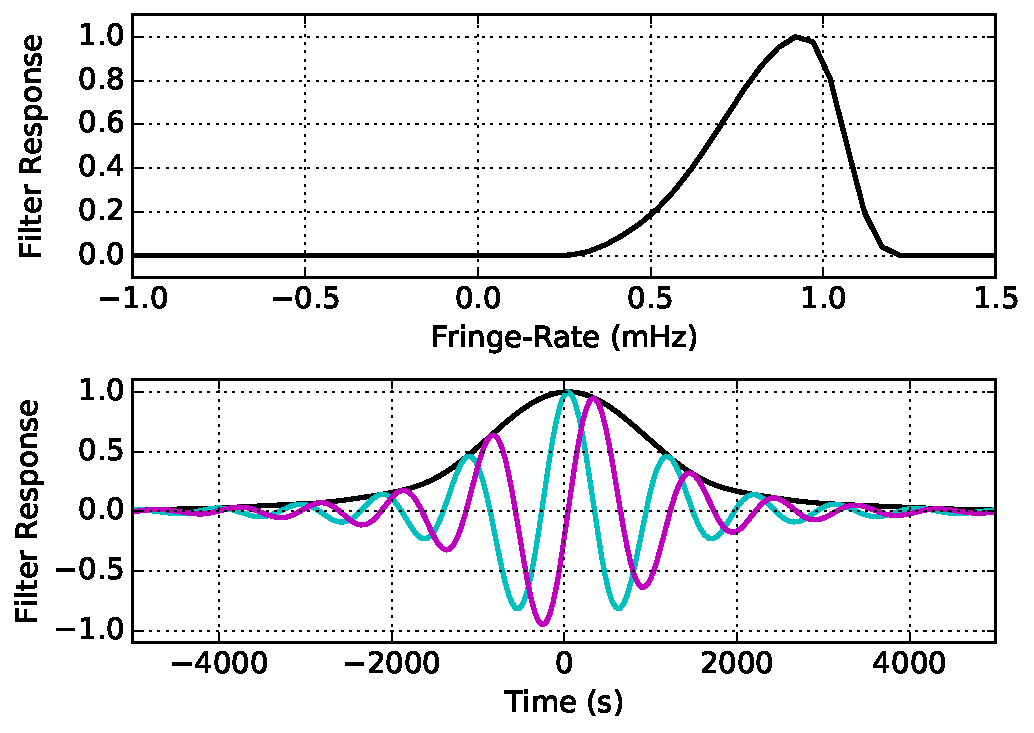
\includegraphics[width=0.75\textwidth]{plots/frp.pdf}
    \caption{Top: the normalized optimal power-spectrum sensitivity weighting in fringe-rate space for our fiducial baseline and 
Stokes I polarization beam. Bottom: the time domain convolution kernel corresponding to the top panel. Real and imaginary 
components are illustrated in cyan and magenta, respectively, with the absolute amplitude in black. The fringe-rate filter acts as 
an integration in time, increasing sensitivity but reducing the number of independent samples in the dataset.}
    \label{fig:frp}
\end{figure}

\section{Signal Loss}

\section{Error Estimation}

\section{Bias}

\section{Power Spectrum Limits}






